\documentclass[11pt,a4paper]{article}
\usepackage[paper=a4paper,width=15cm,left=30mm,height=22cm]{geometry}

\usepackage{xltxtra}
\setmainfont[Mapping=tex-text]{Vollkorn}
\usepackage{setspace}
\linespread{1.0}
\setlength{\parskip}{0.5em}
\setlength{\parindent}{0em}

\usepackage[german]{babel}
\usepackage{graphicx}
\usepackage{acronym}

\usepackage{hyperref}
\usepackage[usenames,dvipsnames]{xcolor}
\hypersetup{
    bookmarks=true,
    colorlinks=true,
    linkcolor=NavyBlue,
    citecolor=NavyBlue,
    urlcolor=NavyBlue
}

\bibliographystyle{plain} 
\bibdata{bibliothek}

\begin{document}
\author{Markus Tacker}
\title{Bachelor-Thesis zur Erlangung des akademischen Grades Bachelor of Science – B.Sc.}

\begin{center}

\begin{small}Hochschule RheinMain\\
Fachbereich Design Informatik Medien\\
Studiengang Medieninformatik

\vspace{1cm}

Bachelor-Thesis\\
zur Erlangung des akademischen Grades\\
Bachelor of Science – B.Sc.\end{small}

\vspace{2cm}

\begin{huge}Konzept und Entwurf eines workflowgesteuerten Systems zur Verwaltung von Texten in Medienprodukten\end{huge}

\end{center}

\linespread{1.25}

\vspace{10cm}

\begin{tabular}{@{}l l}
vorgelegt von & Markus Tacker\\
am & \today\\
& \\
Referent: & Prof. Dr. Jörg Berdux\\
Korreferent: & Prof. Thomas Steffen
\end{tabular}

\pagebreak

\section*{Erklärung gem. ABPO, Ziff. 6.4.3}

Ich versichere, dass ich die Bachelor-Thesis selbständig verfasst und keine anderen als
die angegebenen Hilfsmittel benutzt habe.

\vspace{2cm}

\begin{tabular*}{\textwidth}{@{\extracolsep{\fill}}l r@{}}
Offenbach am Main, \today & Markus Tacker
\end{tabular*}

\vspace{6cm}

\section*{Verbreitung}

Hiermit erkläre ich mein Einverständnis mit den im folgenden aufgeführten
Verbreitungsformen dieser Bachelor-Thesis:

\begin{tabular*}{\textwidth}{@{\extracolsep{\fill}}l r@{}}
Einstellung der Arbeit in die Hochschulbibliothek mit Datenträger: & nein \\
Einstellung der Arbeit in die Hochschulbibliothek ohne Datenträger: & nein \\
Veröffentlichung des Titels der Arbeit im Internet: & ja \\
Veröffentlichung der Arbeit im Internet: & nein
\end{tabular*}

\vspace{2cm}

\begin{tabular*}{\textwidth}{@{\extracolsep{\fill}}l r@{}}
Offenbach am Main, \today & Markus Tacker
\end{tabular*}

\pagebreak

\section*{Danksagung}

\pagebreak

\tableofcontents

\pagebreak

\section{Abstract}

\emph{Das Problem:} Nahezu alle Medien haben eines gemeinsam; sie beinhalten Text. Am Entstehungsprozess dieser Texte sind viele Personen beteiligt. Für diesen Prozess gibt es bisher jedoch kein System, mit der die Verwaltung dieses Vorganges leicht handhabbar ist.

\emph{Die Lösung:} Diese Bachelor-Thesis stellt ein passgenauen Werkzeug vor, das für Texte in Medienprodukten die Zusammenstellung, Organisation, Rechtschreibprüfung, Abnahmen durch den Kunden, Übersetzung, Versionierung und Übergabe in die Produktion erledigt.

Nahezu alle Medien haben eines gemeinsam: Sie beinhalten Text. Für die Verwaltung von Texten bei Medienprojekten gibt es bisher keine ausgereifte Lösung – obwohl bei der Erstellung von Texten sehr viele Personen beteiligt sind, werden Texte in der Regel mit Office-Dokumenten verwaltet, meistens mit Word, vor allem bei großen Projekten kommt Excel zu Einsatz. Der Workflow von einem Bearbeiter zum nächsten erfolgt über den Austausch des Office-Dokumentes via E-Mail, Netzlaufwerk, File-Sharing-Anbieter (z.B. Dropbox) oder Ticketsystem. Dieser Prozess ist aufwendig und fehleranfällig. Sobald mehrere Personen gleichzeitig an den Texten arbeiten, wird manuelles Eingreifen notwendig um die gemachten Änderungen zusammenzuführen. Aufgrund der Vielzahl der am Text beteiligten Personen sind Office-Dateien ein denkbar schlecht geeignetes Mittel um Texte und ihre Änderungen sauber und nachvollziehbar zu verwalten. Auch das Übertragen von Texten aus Office-Dokumenten ist eine Fehlerquelle – es ist stupides Copy\&Paste. In den meisten Fällen müssen dabei im Dokument vorgenommene Formatierungen wie Umbrüche und Absätze entfernt werden um eine saubere Darstellung auf dem Endprodukt zu gewährleisten.

Während der Umsetzung eines Projektes ist besonders Text der Bestandteil des fertigen Produktes, der oft bis zur letzten Minute geändert wird – egal wie viel Aufwand vorher in die Planung geflossen sind. Dies liegt unter anderem daran, dass Text im Gegensatz zu Grafiken, Fotos und anderen Multimedia-Elementen als einziger Informationsträger eindeutig ist und üblicherweise keinen Interpretationsspielraum offen lassen soll. So bietet er auch aus rechtlicher Sicht den problematischsten Bestandteil eines Medienproduktes. In Zeiten, in denen Konkurrenten jede Veröffentlichung der Konkurrenz von Anwälten begutachten lassen sind auch Kunden hier besonders vorsichtig – leider werden aber Texte üblicherweise erst sehr spät den Anwälten des Kunden vorgelegt und deren Expertise lässt sich zeitlich selten in den Projektablauf einplanen. Ein anderes typisches Beispiel für Text-Änderungen in letzter Minute sind Gewinnspiele und andere Angaben mit festen Terminen: Verzögern sich Projekte in der Umsetzung, müssen auch Gewinnspieltermine verschoben werden. 

\begin{figure}[htb]
\begin{center}
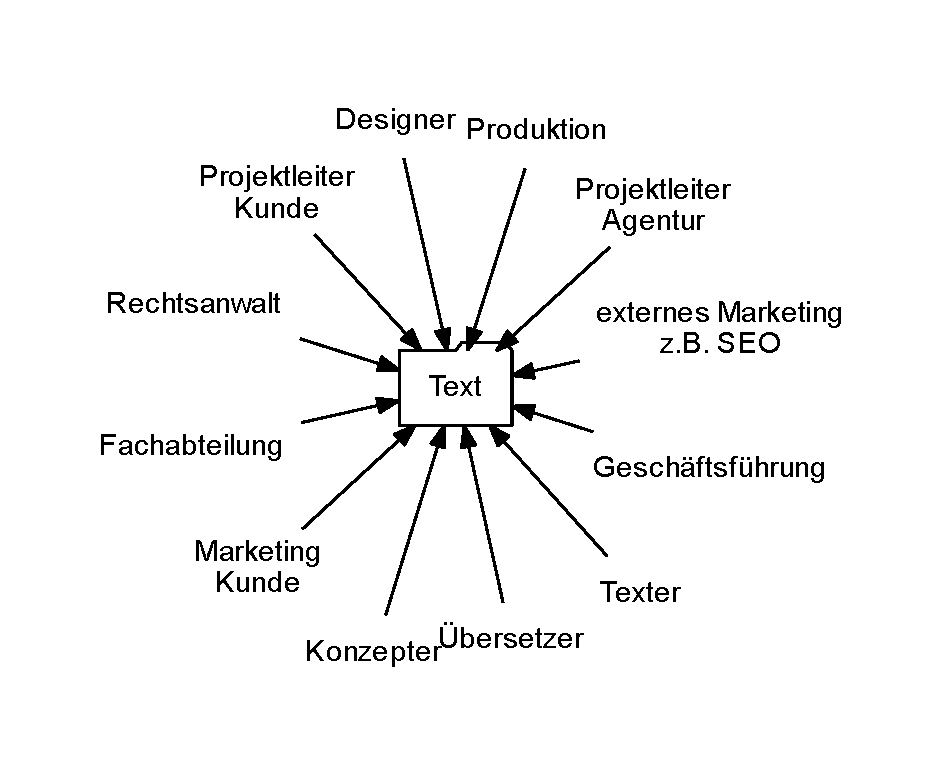
\includegraphics[width=\textwidth]{media/chart-2.pdf}
\end{center}
\caption{Bei der Erstellung von Texten für Medienprodukte beteiligte Personen}
\label{chart:2}
\end{figure}

Da es Kunden aus dem Büroalltag gewöhnt sind, mit Texten umzugehen und sie aus eigener Erfahrung wissen „dass Texte schnell geändert sind“, haben Sie die naive Erwartung, dass die Texte im Endprodukt bis zum Schluss ohne großen Aufwand geändert werden können. Doch gerade bei Text betreffen solche Änderungen viele Beteiligte, die alle informiert werden müssen damit die Änderungen korrekt übernommen werden können.

In dieser Bachelor-Thesis wird ein Workflow entwickelt, der diese Probleme beseitigt und in Form einer browser-basierte Anwendung umgesetzt, auf die alle Beteiligten über ihren Desktop-PC oder ihr Smartphone jederzeit Zugriff haben. Dadurch, dass die Anwendung über das Internet zugänglich ist, können auch Mitarbeitern im Home-Office oder freie Mitarbeiter am Projekt direkt mitarbeiten.

Innerhalb der Anwendung wird das Projekt angelegt und die dafür benötigten Textbausteine definiert. Hierbei können detaillierte Angaben zu deren Eigenschaften gemacht werden, z.B. über den Verwendungszweck oder die maximal Länge. Die einzelnen Textbausteine werden bei diesem Vorgang entsprechend dem Aufbau des Endproduktes in eine Reihenfolge gebracht und hierarchisch angeordnet. So wird eine leichte Orientierung und Zuordnung der Text zum Endprodukt möglich. 

Nachdem die benötigten Textbausteine definiert wurden, werden diese durch Texter befüllt. Für Texter stellt die Anwendung Hilfsfunktionen zur Verfügung. Dazu zählen Informationen wie Zeichenlänge und Wortanzahl und Rechtschreibkorrektur mit Wörterbuch.

Sobald die Texte hinterlegt wurden durchlaufen sie die Qualitätskontrolle durch andere Mitarbeiter des Projektes und anschließend den Freigabeprozess beim Kunden. Wurden die Texte freigegeben, können die zusammengestellten Texte in das Endprodukt übernommen werden. 

Alle Vorgänge werden innerhalb der Anwendung protokolliert und sind so für jeden Beteiligten leicht nachvollziehbar. Aufgaben können automatisch aufgrund von Änderungen erzeugt werden, oder von Mitarbeiter angelegt werden. So wird sichergestellt, dass alle Projektmitarbeiter jederzeit über ihre Aufgaben bezüglich der Texte informiert sind, bei Änderungen die verantwortlichen Mitarbeiter informiert werden. Dadurch wird es möglich auch bei Korrekturen in letzter Minute diese Änderungen gezielt und transparent zu übernehmen.

\section{Problem-Analyse}

\subsection{Definition}

was sind „Texte in Medienprodukten“

\subsection{Die besondere Rolle von Text}

Fast jedes Multimedia-Produkt enthält Text, denn Text ist im Gegensatz zu Grafiken, Fotos oder Animationen ein eindeutiger Informationsträger und unterliegt viel weniger stark einer Intepretation durch den Rezipienten eines Mediums als die symbolisierte oder stilisierte Darstellung von Informationen in audiovisuellen Medien. Auch aus rechtlichen Aspekten ist Text aus den genannten Gründen der einzige verbindliche Informationsträger – bestes Beispiel hierfür ist das sogenannte „Kleingedruckte“, dass sich gerade bei inhaltlich sehr stark komprimierten Werbeformen, wie z.B. Plakat- oder Fernsehwerbung, findet.

Ist die Textmenge, die im Absatzmarketing zum Einsatz kommt, noch überschaubar, gibt es doch Medienprodukte, deren Hauptbestandteil Text ist. Hierunter fallen klassische Druckerzeugnisse wie Broschüren und Kataloge oder Produkte der Unternehmenskommunikation wie Jahresberichte und Pressemeldungen. Doch besonders digitale Medienprodukte werden oft mit großen Textmengen versehen – von der einfachen Produkt-Microsite, über Werbmittel wie Newsletter bis zur Unternehmenswebsite – die Möglichkeit Inhalte hierarchisch zu struktuieren und sogar über eine Suche zugänglich zu machen hebt eine Limitierung des Umfanges, wie bei Druckprodukten, praktisch auf.

\subsection{Erstellung von Texten in Projekten}

Alle genannten Produkte haben gemeinsam, dass ihre Erstellung in der Regel die Zusammenarbeit vieler Personen erforderlich macht. Beobachtet man den Prozess, kann man feststellen, dass es sechs verschiedene Rollen rund um die Texterstellung gibt, die ein Mitarbeiter einnehmen kann; zum Teil übernimmt eine Person dabei auch die Aufgaben mehrerer Rollen:

\begin{enumerate}
\item{Der \textbf{Informationsarchitekt} (oder Konzepter) legt die Struktur eines Produktes fest und damit auch die Art und Menge des benötigten Textes,}
\item{der \textbf{Texter} verfasst die Texte,}
\item{der \textbf{Übersetzer} überträgt die Texte in weitere Sprachen,}
\item{der \textbf{Qualitätsmanager} überwacht die Ergebnisse der Prozesse,}
\item{der \textbf{Produktbesitzer} (oder Kunde) ist für die fachlichen und rechtliche Aspekte, sowie das Festlegen der zeitlichen Rahmenbedingungen verantwortlich,}
\item{der \textbf{Produzent} ist für die Erstellung des eigentlichen Produktes verantwortlich.}
\end{enumerate}

Alle Rollen haben im Verlauf eines Projekts, zu unterschiedlichen Zeiten und mit unterschiedlichem Gewicht, Einfluss auf die Gestaltung der Texte. Es existieren auch Abhängigkeiten zwischen den Rollen, so kann ein Übersetzer erst arbeiten, wenn der Text vorliegt und vom Produktbesitzer abgenommen wurde; wird aber zu einem späteren Zeitpunkt der Text geändert, muss auch wieder der Übersetzer neu beginnen.

Neben den menschlichen Einflüssen gibt es auch projektbedingte Einflüsse auf Text. Zum einen gibt es Situationen in denen in Texten bestimmte Informationen enthalten sind, die einen zeitlichen Aspekt abbilden. Ein Bespiel sind Gewinnspiele: Verschieben sich durch Probleme während dem Projekt die Zeiten, ab wann ein Produkt beim Rezipienten vorliegt, müssen auch evtl. knapp kalkulierte Gewinnspieltermine angepasst werden. Des weiteren gibt es oft erst gegen Ende eines Projektes Textänderungen aus der Rechtsabteilung des Kunden, da aus zeitlichen und finanziellen Gründen Anwälte gerne erst dann konsultiert werden, wenn Projekte kurz vor der Fertigstellung stehen. Da es Kunden von den Office-Produkten her gewöhnt sind, mit Text umzugehen, und sie aus eigener Erfahrung vermeintlich wissen dass Texte schnell geändert sind, erwarten sie auch, dass die Texte im Produkt bis zum Schluss geändert werden können.

\subsection{Textspezifische Aufgaben}

\begin{figure}[htb]
\begin{center}
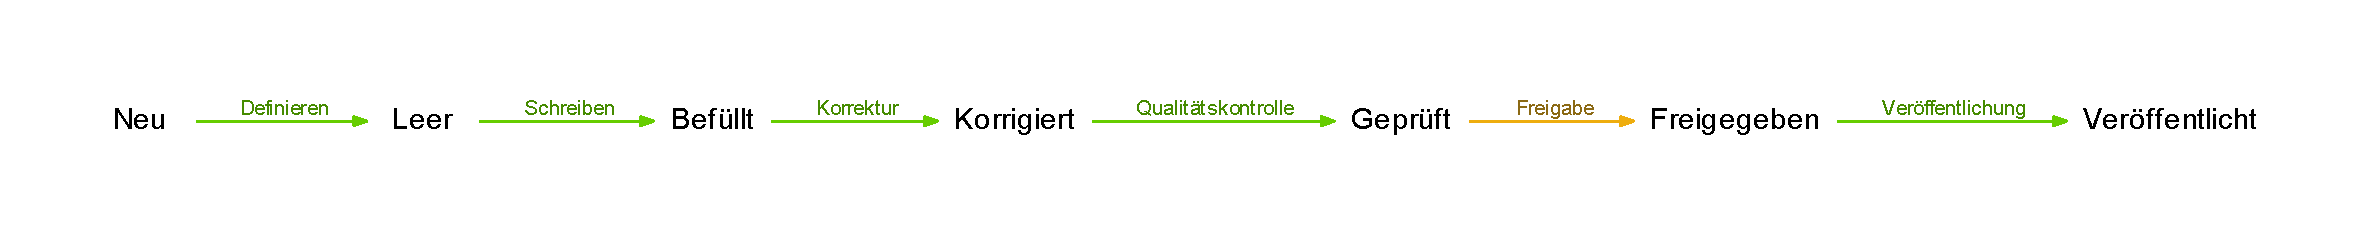
\includegraphics[width=\textwidth]{media/chart-3.pdf}
\end{center}
\caption{Operationen bei der Erstellung von Texten}
\label{chart:3}
\end{figure}

Betrachtet man die Arbeiten in Zusammenhang mit Text lassen sich diese in 6 eigenständige Operationen unterteilen:

\begin{enumerate}
\item{Durch \textbf{Definieren eines Textbausteines} wird festgelegt, wie der benötigte Text beschaffen sein muss. Die Aussage „Wir brauchen an dieser Stelle eine Überschrift“ ist ein Beispiel für diese Operation. Sie legt fest, wie der Textbausteine gestaltet werden muss, um die ihm zugedachte Aufgabe zu erfüllen. Neben der Angabe zur Platzierung auf dem Medienprodukt durch „an dieser Stelle“ wird implizit durch „eine Überschrift“ eine Angabe zur inhaltlichen und visuellen Gestaltung getroffen; Überschriften sollen kurz und knapp sein und ihre visuelle Gestaltung wird durch den Styleguide des Projektes festgelegt.}
\item{Das \textbf{Schreiben eines Textes} befüllt einen Textbaustein mit einem Text in einer Sprache. Bei diesem Vorgang wird der Text entsprechend der Vorgabe aus der Beschreibung als Original erstellt oder aus Quellen außerhalb des Projektes kopiert und eingefügt. }
\item{In der \textbf{Korrektur} wird der Text inhaltlich und grammatikalisch überprüft und entsprechend angepasst. Der Korrektor muss dabei für eine grammatikalische Überprüfung des Textes kein Fachwissen bezogen auf das Projekt haben. Ist diese Fachwissen vorhanden, kann eine inhaltliche Korrektur vorgenommen werden.}
\item{In der \textbf{Qualitätskontrolle} wird der Text dahingehend überprüft, ob er den Anforderungen gemäß der Beschreibung und inhaltlichen Vorgaben, auch hinsichtlich des gesamten Projektes entspricht. }
\item{Durch die \textbf{Freigabe} wird der Text abgenommen und kann nun in das Endprodukt übernommen werden.}
\item{Durch die \textbf{Veröffentlichung} wird der Text in das Endprodukt eingebracht.}
\end{enumerate}

\begin{figure}[htb]
\begin{center}
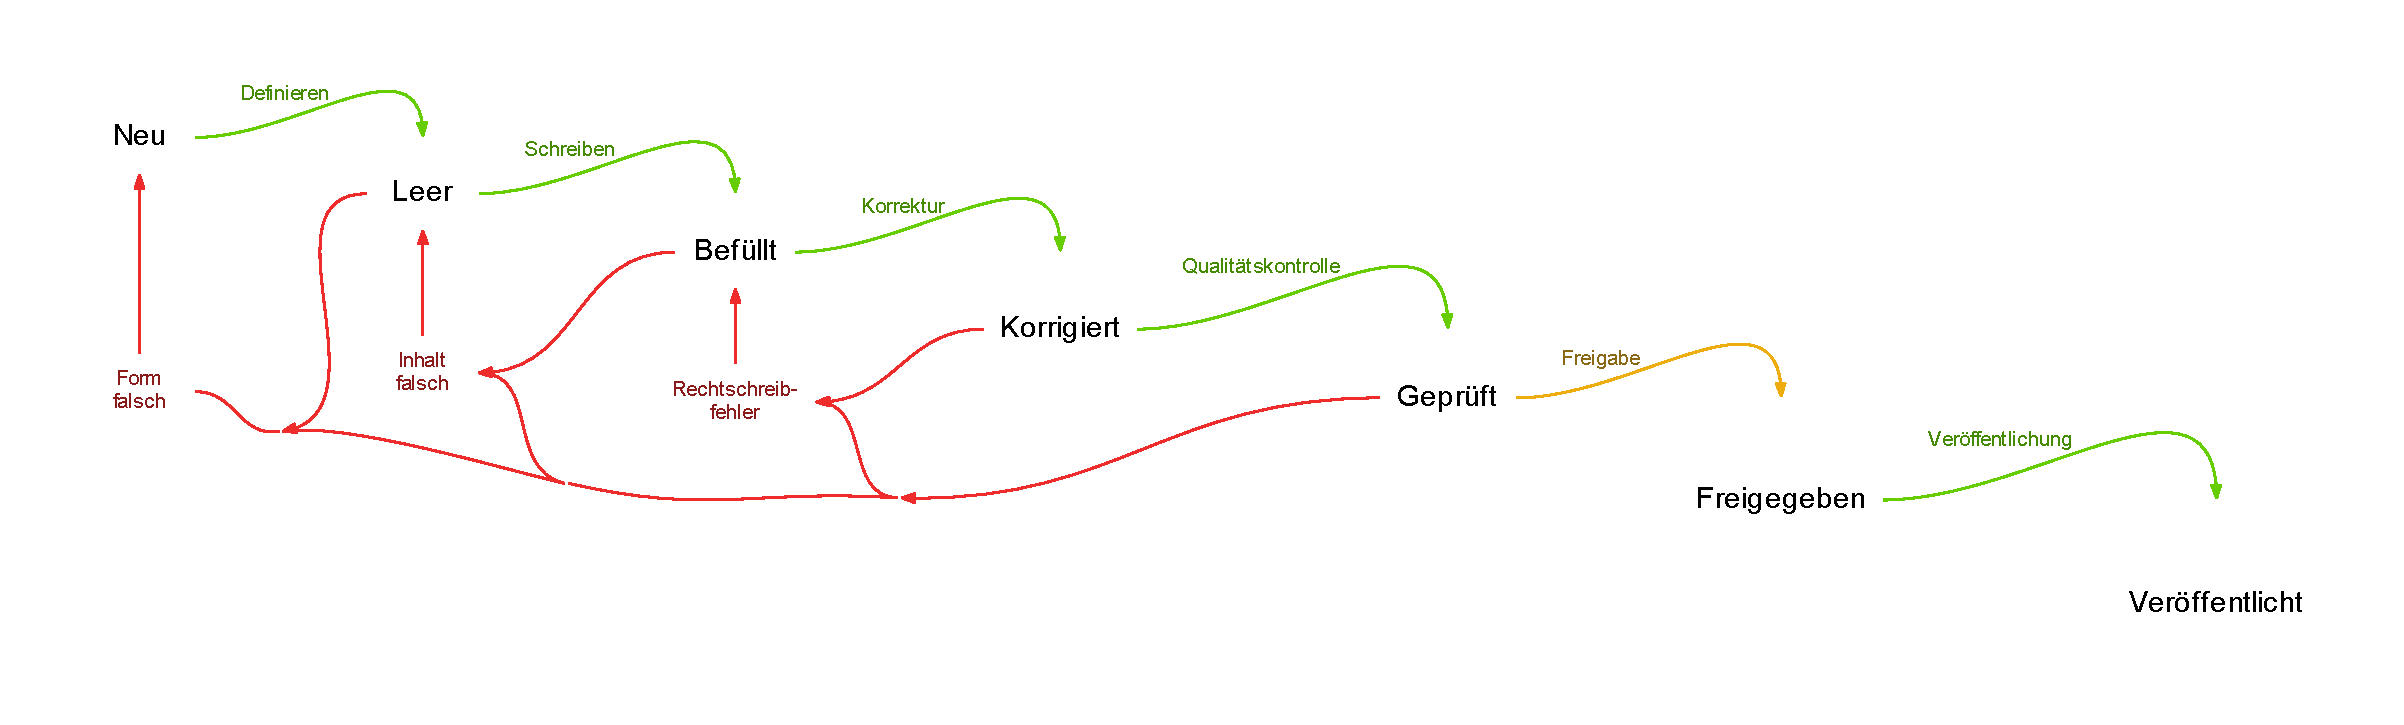
\includegraphics[width=\textwidth]{media/chart-4.pdf}
\end{center}
\caption{Operationen bei der Erstellung von Texten mit Qualitätskontrolle}
\label{chart:4}
\end{figure}

Diese Operationen werden auch 1:1 auf die übersetzte Version eines Textes angewendet.

\begin{figure}[htb]
\begin{center}
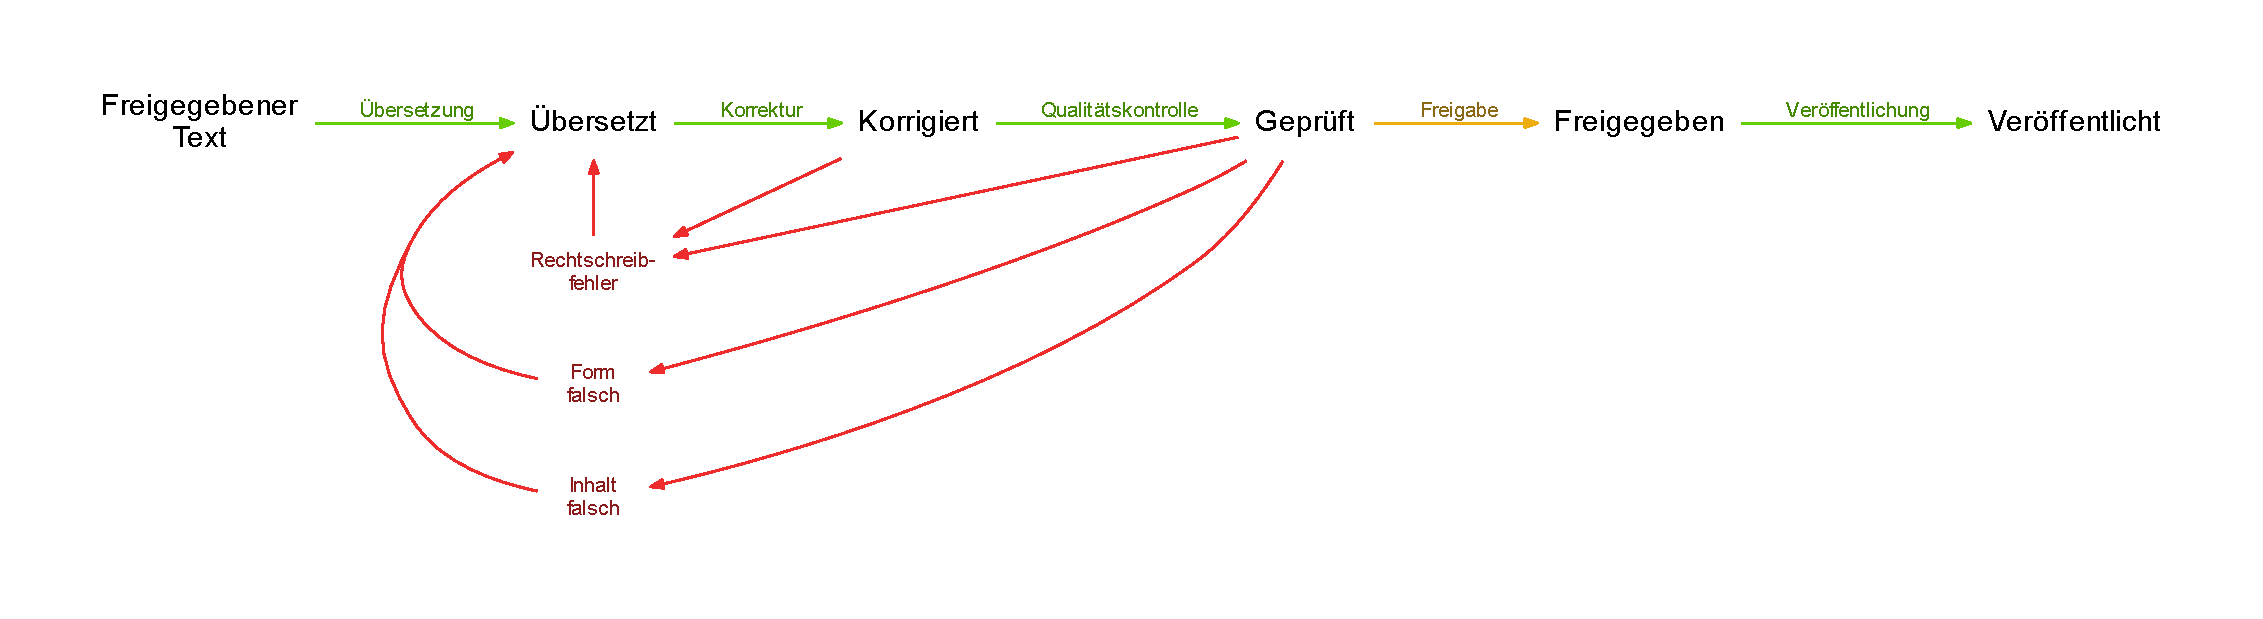
\includegraphics[width=\textwidth]{media/chart-5.pdf}
\end{center}
\caption{Operationen bei der Übersetzung von Texten mit Qualitätskontrolle}
\label{chart:5}
\end{figure}

\subsection{Microsoft Office als Standard}

\subsection{Word und Excel sind „leichtgewichtige“ Werkzeuge}

So komplex auch die Abläufe bei der Erstellung von Texten für Medienprodukte sind, um so erstaunlicher ist die Tatsache, dass das Werkzeug der Wahl zur Abbildung dieser Prozesse in den allermeisten Fällen \emph{Microsoft Word} oder \emph{Excel} ist. Auf den ersten Blick bilden diese Werkzeuge viele der benötigten Funktionen rund um die Textprozesse ab, aber im alltäglichen Gebrauch treten viele Probleme gerade im Bereich des gemeinsamen Bearbeitens, paralleler oder nachträglicher Änderungen und der Übertragung der fertigen Texte in den Produktionsprozess auf. Der Grund für die Wahl der \emph{Office}-Produkte liegt auf der Hand: sind sie doch in den allermeisten Unternehmen der Standard zur Textverarbeitung und sogar plattformunabhängig verfügbar – zumindest existiert die Möglichkeit das Microsoft Office-Dateiformat auf allen Platformen zu bearbeiten. Da bei allen Projektbeteiligten eine Installation von \emph{Microsoft Office} vorausgesetzt werden kann, werden sie zu „leichtgewichtige“ Werkzeugen, die vom Anwender keine zusätzlichen Aufwände z.B. bei der Installation oder Eingewöhnung erfordern. Selbst auf Plattformen, die von \emph{Microsoft Office} nicht offiziell unterstützt werden (z.B. Linux) existieren Programme mit denen das Office-Dokumenten-Format geöffnet und bearbeitet werden kann.

\subsection{Die verwendeten Office-Funktionen}

Als klassisches Textverarbeitungsprogramm verfügen Office-Programme über viele Funktionen, die die Erstellung von Texten erleichtern.

\begin{itemize}
\item{Rechtschreibkorrektur für alle üblichen Sprachen}
\item{Kommentarfunktion}
\item{Änderungsfunktionen (Nachverfolgen, wer was geändert hat)}
\item{Möglichkeit zur hierarchischen Strukturierung der Texte in Seiten, Kapitel und Abschnitte}
\item{Möglichkeit zum Anlegen eines Inhaltsverzeichnisses (in Word)}
\item{die tabellarische Ansicht in Excel ermöglicht eine übersichtliche Darstellung, meist mit der Originalsprache in der ganz linken Spalte, pro Zeile ein Text, die Übersetzungen dann in den weiteren Spalten}
\item{Export-Funktion nach PDF}
\item{Globales Suchen und Ersetzen}
\item{Formatierungsfunktionen (fett, kursiv, farblich) zum Hervorheben von wichtigen Passagen oder Markieren von Todos, etc.}
\item{Setzen von Hyperlinks (für Web-Projekte)}
\end{itemize}

Office-Dateien sind einfach auszutauschen – in Unternehmen werden die Dateien in der Regel auf einem Netzwerk-Laufwerk gespeichert. Zum Bearbeiten legt man sich eine lokale Kopie an und arbeitet in dieser Datei. Anschließend kopiert man die neue Version, meist unter Einhaltung eines bestimmten Benamungsschemas, wieder auf dem Netzlaufwerk ab. Hier können Konflikte auftreten (wenn zwei Personen gleichzeitig an der selben Datei arbeiten), diese müssen dann manuell gelöst werden. Wird die Datei direkt vom Netzlaufwerk geöffnet wird diese gesperrt und kann nur von einer Person bearbeitet werden.

Aufgrund der scheinbaren Vorteile der Office-Suite wird diese zu Beginn eines Projektes als geeignet angesehen und als Werkzeug für die Erfassung, Definition und Übersetzung der Texte eines Projektes ausgewählt.

Die im Verlauf des Projekts auftauchenden Probleme werden dann als gegeben akzeptiert, da man „nun“ damit zurecht kommen muss, um den Verlauf des Projektes nicht zu verzögern. Bei neuen Projekten wird aber die gleiche Entscheidung wieder getroffen.

\subsection{Office-Programme sind die falschen Werkzeuge}

Der Grund, warum Office-Programme wie \emph{Word} und \emph{Excel} verwendet werden ist der, dass keine keine dedizierten Lösungen existieren, die explizit die genannten Abläufe in der Textverarbeitung abbildet. Es existieren vielen Produkte aus dem Bereich der Projektverwaltungswerkzeuge, Mediendatenbanken oder Content-Management-Systemen die die Prozesse rund um die Erstellung von Medienprodukten vereinfachen, aber keine kann die genannten Probleme und Abläufe zufriedenstellend abbilden.

\subsection{Beispiele aus der Praxis}

Die Analyse des Problems basiert auf Interviews mit Menschen, die in ihrem Arbeitsalltag regelmäßig mit Texten zu tun haben. In diesen Interviews wurden die Personen nach ihren Erfahrungen in der Projektarbeit bezüglich Texten befragt und gebeten die aus ihrer Sicht am häufigsten auftretenden Probleme zu nennen.

\subsubsection{MAN Truck \& Bus AG: Texte für mobile Vertriebssoftware}

Markus Rüb ist als Projektleiter bei der MAN Truck \& Bus AG mit der Einführung von Tablet PCs als Vertriebshilfsmittel betraut.

\subsection{Schlussfolgerung}

\section{Konzeption eines an die spezifischen Probleme angepassten Workflows}

\subsection{Vorraussetzung / Abgrenzung}

\subsection{Workflow}

Beschreibung des optimalen Workflows und die Rolle der Beteiligten

\subsection{Beschreibung der notwendigen Funktionalität}

Unterteilung in Muss- und Kann-Kriterien

\subsection{Nachteile/Risiken des Konzepts}

\subsection{Personas}

Vorstellung (basierend auf Interviews mit realen Personen), Analyse des Konzepts in Bezug auf Personas

\subsubsection{Texter}

\section{Entwurf einer Anwendung}

Diese vier Leitlinien repräsentieren die Grundgedanken bei der Entwicklung von \textbf{re:text}:

\begin{itemize}
\item{Das wichtigste zuerst: Die aktuelle Aufgabe soll immer im Fokus der Darstellung liegen.}
\item{Schnell zum Ziel: Alle Aufgaben müssen leicht und umkompliziert durchführbar sein.}
\item{Nicht nerven: Ständige Benachrichtigungen lenken ab und müssen deswegen so gestaltet sein, dass diese sich nach den Präferenzen des Nutzers richten.}
\item{Hilfe nur einen Klick entfernt: Das Hilfesystem muss kontextsensitiv verfügbar sein und ist eine Kernfunktion der Anwendung}
\end{itemize}

\subsection{Überblick}

Diese Abbildung liefert einen Überblick über den Aufbau des Systems:

\begin{figure}[htb]
\begin{center}
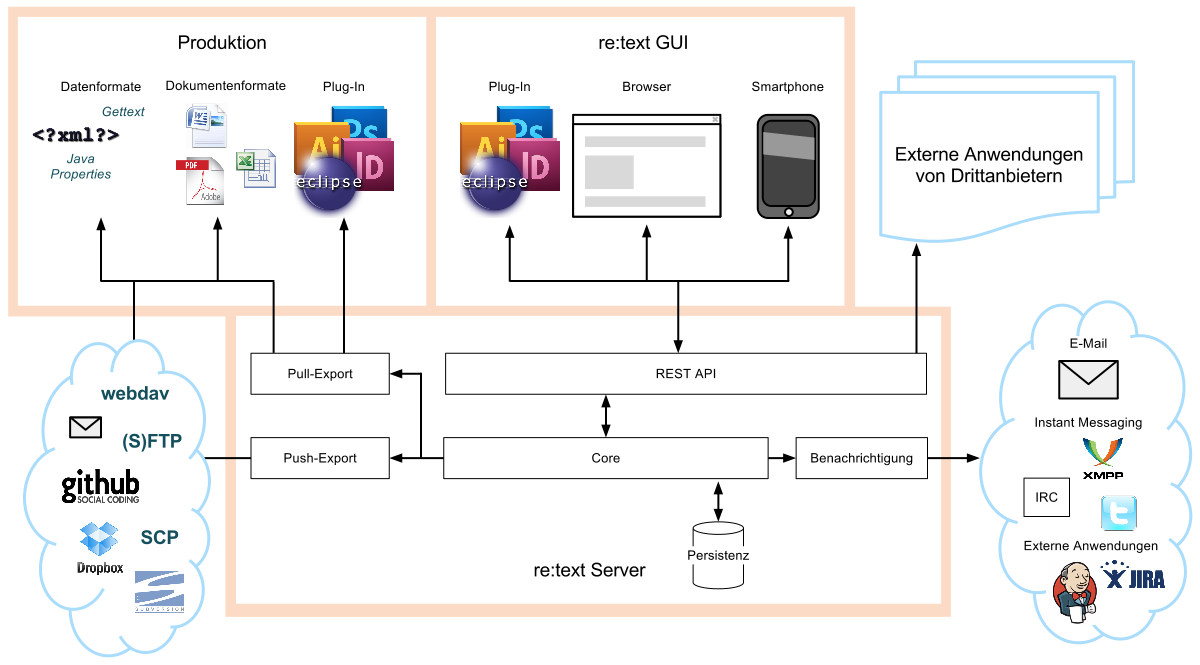
\includegraphics[width=\textwidth]{media/System.pdf}
\caption{Aufbau des Systems}
\label{chart:1}
\end{center}
\end{figure}

Die Zentrale Komponente von \textbf{re:text} bildet der Server. Für die Benutzer erfolgt der Zugriff mit Hilfe einer GUI, die mit der REST-API des Servers kommuniziert. In der ersten Version wird eine browserbasierte GUI auf Basis von HTML5 und JavaScript existieren, die auch schon auf Smartphones verwendet werden kann. Später kommen dann spezielle Plugins für Adobe-Produkte und weitere wichtige Produktionsumgebungen hinzu. Auch native GUIs für Smartphones verwenden die gleiche API. Die Schnittstellen können auch von Drittanbietern dazu verwendet werden, eigenen Clients für das System zu entwickeln. In die Endprodukte gelangen die Texten über den Export, exportiert wird dabei in viele Formate, neben Datenformaten wie z.B. XML werden auch Dokumentenformate wie z.B. Word exportiert. Der Export kann durch den Anwender erzeugt werden (\emph{Pull-Export}), aber auch automatisch, z.B. nach festgelegten Zeitplänen oder Ereignissen erfolgen. Dieser \emph{Push-Export} erfolgt auf je nach Projekt festlegbaren Orte, wie z.B. FTP-Server oder Versionsverwaltungssysteme. Die Benachrichtigungen über Aufgaben und Änderungen an Texten kann via E-Mail, aber auch mittels Instant-Messaging-Systeme oder durch den Aufruf fremde API-Endpunkte erfolgen – dies ist ebenfalls innerhalb eines Projektes und pro Nutzer individuell konfigurierbar.

\subsection{Schnittstellen}

Anforderungen, Umfang, Ausprägung für Import-, Export- und Benachrichtigungsschnittstellen

\subsection{Grundüberlegung zu einer GUI}

Anforderungen, Grundsätze, Usability, Aufbau, Wireframes

\section{Implementierung des Konzepts}

\subsection{Abgrenzung}
\subsection{Beschreibung der gewählten Umsetzung, Komponenten}

\subsection{Anwendung der Umsetzung am Beispiel des Studiengangsflyers}

\section{Fazit}

\pagebreak

\bibliography{bibliothek}

\end{document}